\begin{strip}
\centering
\vspace{-1.2em}
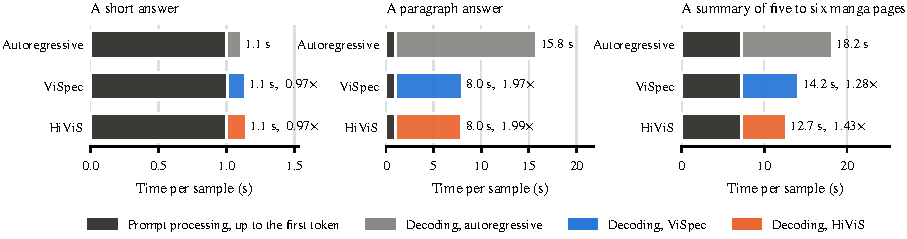
\includegraphics{figures/teaser.pdf}
\captionsetup{hypcap=false}
\captionof{figure}{\textbf{Where the time of one sample goes.} Mean time per sample on \qwenL for autoregressive decoding and for two speculative decoders built for vision-language models, \vispec and \hivis, split at the first output token. The speedup over autoregressive decoding follows each total. Short answers are TextVQA answers of a word or phrase, paragraphs are long TextVQA answers, and each manga window holds five or six pages of \rvp. Each panel is one GPU job.}
\captionsetup{hypcap=true}
\label{fig:teaser}
\vspace{-0.6em}
\end{strip}
